% This file is part of the Platypus project.
% Copyright 2016 the authors.

% to-do
% - write discussion section w MKN input
% - fix all remaining occurrences of ARC, MKN, HWR, DWH, or CITE
% - submit to journal and arXiv
% - forward to Freeman, Bovy, others?

% style notes
% - never use \cite{}, always \citep{} or \citealt{}.

\documentclass[12pt, letterpaper, preprint]{aastex}

% text shit
\newcommand{\acronym}[1]{{\small{#1}}}
\newcommand{\project}[1]{\textsl{#1}}
\newcommand{\sdssiii}{\project{\acronym{SDSS-III}}}
\newcommand{\apogee}{\project{\acronym{APOGEE}}}
\newcommand{\aspcap}{\project{\acronym{ASPCAP}}}
\newcommand{\gaiaeso}{\project{Gaia--\acronym{ESO}}}
\newcommand{\galah}{\project{\acronym{GALAH}}}
\newcommand{\thecannon}{\project{The~Cannon}}
\newcommand{\foreign}[1]{\textsl{#1}}
\newcommand{\eg}{\foreign{e.\,g.}}
\newcommand{\etal}{\foreign{et\,al.}}
\newcommand{\documentname}{\textsl{Article}}
\newcommand{\sectionname}{Section}

% math shit
\newcommand{\teff}{T_{\mathrm{eff}}}
\newcommand{\logg}{\log g}

% figure shit
\newlength{\figwidth}\setlength{\figwidth}{0.3\textwidth}
\newcommand{\insanefigure}[1]{%
\includegraphics[width=\figwidth]{./figs/#1_MgFe.png}%
\includegraphics[width=\figwidth]{./figs/#1_MgK.png}%
\includegraphics[width=\figwidth]{./figs/#1_AlMg.png}\\
\includegraphics[width=\figwidth]{./figs/#1_NaO.png}%
\includegraphics[width=\figwidth]{./figs/#1_CN.png}%
\includegraphics[width=\figwidth]{./figs/#1_SAl.png}\\
\includegraphics[width=2\figwidth]{./figs/#1_gal.png}%
\includegraphics[width=\figwidth]{./figs/#1_HR.png}\\
\includegraphics[width=2\figwidth]{./figs/#1_vlon.png}}

% results shit
\newcommand{\totalnumber}{98462}

\begin{document}\sloppy\sloppypar

\title{Chemical tagging can work: \\
       Identification of stellar phase-space structures \\
       purely by chemical-abundance similarity}
\author{David~W.~Hogg\altaffilmark{1,2,3,4},
        Andrew~R.~Casey\altaffilmark{5},
        Melissa~K.~Ness\altaffilmark{4},
        Hans-Walter~Rix\altaffilmark{4},
    and~Daniel~Foreman-Mackey\altaffilmark{6}}
\altaffiltext{1}{Simons Center for Data Analysis, 160 Fifth Avenue, 7th Floor, New York, NY 10010, USA}
\altaffiltext{2}{Center for Cosmology and Particle Physics, Department of Phyics,
  New York University, 4 Washington Pl., room 424, New York, NY, 10003, USA}
\altaffiltext{3}{Center for Data Science, New York University, 726 Broadway, 7th Floor, New York, NY 10003, USA}
\altaffiltext{4}{Max-Planck-Institut f\"ur Astronomie, K\"onigstuhl 17, D-69117 Heidelberg, Germany}
\altaffiltext{5}{Institute of Astronomy, University of Cambridge, Madingley Road, Cambridge CB3~0HA, UK}
\altaffiltext{6}{Department of Astronomy, University of Washington, Box 351580, Seattle, WA 98195-1580}
\email{david.hogg@nyu.edu}

\begin{abstract}
% Context:
The chemical-tagging hypothesis is that every star ought to carry---%
in its detailed chemical abundances---%
an informative signature of its molecular-cloud birth location and time.
This idea has not previously yielded scientific successes, probably because of the
noise and incompleteness in chemical-abundance measurements.
However, we have succeeded in substantially improving spectroscopic measurements with \thecannon\ 
(now delivering individual abundances with precisions around 0.04~dex).
% Aims:
We test the chemical-tagging hypothesis by looking at clusters in abundance space
and confirming that they are clustered in phase space.
% Methods:
We identify (by the k-means algorithm) overdensities of stars observed by the \apogee\ spectroscopic survey
in a 15-dimensional chemical-abundance space delivered by \thecannon,
and plot the associated stars in phase space.
We use \emph{only} abundance-space information (no positional information) to identify stellar groups.
% Results:
We find that clusters in abundance space are indeed clusters in phase space.
We recover some known clusters and find other interesting structures.
This confirms the chemical-tagging hypothesis and verifies the precision of abundances delivered by \thecannon.
This is the first-ever project to identify phase-space structures by blind search purely in abundance space;
the prospects for future data sets are very good.
\end{abstract}

\keywords{
  Galaxy: abundances
  ---
  Galaxy: stellar content
  ---
  Galaxy: structure
  ---
  globular clusters: general
  ---
  open clusters and associations: general
  ---
  stars: abundances
}

\clearpage
\section{Introduction}\label{sec:intro}

Ensembles of stars in the Milky Way are born in molecular clouds,
which are presumed to be near-homogeneous in their chemical element
composition.
However, most stars are born in unbound associations, or are born in
star clusters that disperse rapidly; they will eventually end up in
very different parts of phase space, on differing orbits.
Yet, if every star preserved its photospheric element abundances over
its lifetime (at least for most elements), then stars of common birth
origin ought to be identifiable through their detailed photospheric
abundances, long after any spatial or phase-space proximity has
vanished.

This idea, dubbed ``chemical tagging'', was proposed long ago
\citep{freeman} and is one of the principal motivations for a number
of surveys, most notably \apogee\ \citep{apogee},
\gaiaeso\ \citep{gaiaeso} and \galah\ \citep{galah}.
In order to determine the precise abundance labels for chemical
tagging, these surveys are each measuring high-resolution, high
signal-to-noise ($S/N$) spectra for hundreds of thousands of stars across the
Galaxy's disk, bulge and halo.

Chemical tagging holds the promise of revealing not just the
star-formation history of the Galaxy, but also the accretion history
(as things that fall in are expected to be chemically distinct from
those that form in the parent body; for example, \citealt{font}) and
stellar-orbit diffusion process like radial mixing and radial
migration (for example, \citealt{roskar, quillen}).  After
stars are born---or after a star cluster is accreted and
disrupted---associations or groups will disperse, through either
internal two-body processes or external tidal forces.

Although undeniably promising---and motivating the 
launch of costly large-scale spectroscopic surveys---
chemical-tagging as a search technique has yet to be proven in
practice: identifying stars of common birth origin {\it purely} on the
basis of their near-identical abundances patterns, without any
consideration of position or velocity.

Part of the reason that chemical tagging still remains unrealized
is because the level of abundance specificity required
is very high.
If there are thousands of (relevant) molecular clouds forming stars in
the recent history of the Milky Way, clumps of stars can only stand
out in a high-dimensional abundance space: therefore accurate, or at
least precise, measurements of many different abundances are needed
for stellar sibling to have sufficiently unique fingerprints.
Stellar spectroscopic surveys now have the resolution, signal-to-noise,
wavelength coverage, and sample sizes to deliver many different chemical tags for each star.

% ARC to DWH:   "stand out in a high-dimensional abundance space" -->
%		 	    They'll only stand out in a high-dimensional abundance
% 				space, or a low-dimensional abundance space where those
% 				dimensions are all very orthogonal (e.g., different
% 				nucleosynthetic pathways). Should we add anything to that
%				effect?

There are, however, two big issues.
The first is that the physical assumptions behind the idea may require
refinement:
There may be chemical-abundance overlaps among open clusters
\citep{blancocuaresma}; coeval groups of stars may have similar tags
but different birth places \citep{mitschang}, and the
chemical-abundance space might be low in dimensionality.
On the other hand, precise studies of stellar twins \citep{melendez, jofre}
and open clusters \citep{bovy} indicates that chemical abundances ought to be
very precisely similar for co-eval stars.

The second issue for chemical tagging---and the one we address
here---is measurement precision (and accuracy).
The current precision on abundance measurements in the published
survey catalogs is not high enough (for example, \citealt{martell,
  ting}).
However, our recent work \citep{thecannon} suggests that \emph{data}
are precise enough: there is enough signal-to-noise at the relevant
locations in spectrum space to deliver high-precision tags.
The existence of very large data sets, homogeneous in data/spectrum
space, suggest that one can use data-driven approaches to determining
stellar abundances, which can considerably outperform traditional
methods.
These traditional approaches are based on \foreign{ab-initio} physical models
that have shortcomings that become apparent in this age of
high-quality spectra, and the data-analysis methods do not make use of
all of the information in the data sets.
Improving the models and exploiting the entire information
content in the data is critical if we are going to deliver useful
chemical tags.

Our specific contribution in this space has been to develop
\thecannon\ \citep{thecannon, ages}, which is a data-driven model for
stellar spectra.
This model can deliver stellar parameters and chemical abundances for
stars, making use of every pixel of every stellar spectrum (that is,
all the information in the data) but making no use at all of physical
models of stars.
It relies only on there being training data---\emph{some} stars for
which parameters and abundances are known and believed.
In companion papers \citep{casey16, ness16} we show that
\thecannon\ can deliver 15 to 19 abundances for stars in the
\apogee\ survey, at precisions higher than even the training data on
which the model is trained.
We say more about this below.
We will show here that \thecannon\ improves chemical abundance measurements
to the point that \emph{chemical tagging is now possible.}

One note on \emph{accuracy} and \emph{precision:}
In principle, the problem of chemical tagging does not require
absolute accuracy for chemical-abundance measurements.
We only require that we can precisely see that two stars are similar
in their abundances; even if we are wrong about the absolute values of
those abundances.
This point might make it seem like we don't care that our models are
wrong, so long as they are \emph{consistent.}
However, this is a bit misleading:
For chemical tagging to succeed, we need stars with different
atmospheric parameters $(\teff, \logg)$ but the same chemical
abundances to be assigned the same position in chemical-abundance
space.
That doesn't require overall accuracy, but it requires that the models
have the right dependencies on atmospheric parameters such that the
wrongness in abundance space is consistent across the Hertzsprung-Russell diagram.
That is, we need a substantial amount of accuracy to achieve our goals.

It is important to realize that analysis techniques based on \foreign{ab-initio}
physical models are inaccurate, yet they too strive to improve precision
in the face of knowingly inaccurate models.  Incomplete atomic data, 
simplifications of photospheric structure, presumptions about convective
motion, and inconsistencies resulting from assumptions of the local thermal
equilibrium, all contribute to produce knowingly inaccurate abundances.
\thecannon\ stands out because it demonstrably improves the precision on
chemical abundances, whereas the accuracy of those labels is limited only
by the training set employed.

In what follows, we are going to use \apogee\ \acronym{DR12} data \citep{dr12}, in
which we can re-derive 15 element abundances (C, N, O, Na, Mg, Al, Si,
S, K, Ca, Ti, V, Mn, Fe, Ni), using \thecannon\ \citep{thecannon}.
The \apogee\ data set covers a huge radial extent and---because the
data are taken in the infrared---explores the thin disk.
However, it has the disadvantage that it's spatial coverage is incomplete
(i.e., limited pointings produce a \foreign{`swiss cheese'}-like structure),
which makes it hard to see, within the data set, linear or
extended stellar structures.
In many ways, \galah\ will deliver improvements, both because it will
have more abundances (possibly 29) and contiguous sky coverage.

One final note:
we think of this \documentname\ as performing a proof of concept.
We know that the stellar members of open and globular clusters---stars
that are identified by being close in phase space---contain highly
informative abundance information that identifies them also in
chemical-abundance space.  Does this work the other way around? 
Can chemical tagging identify small subsets of stars, among a vastly
greater background sample, that have a common birth origin? If we 
find stars purely by their clustering in abundance space and subsequently
show that they are part of a still spatially coherent cluster, then
we will have resolved all practical outstanding issues plaguing 
chemical tagging, thereby coming closer to the tantalizing potential 
in truly unravelling the formation of the Milky Way.

\section{Data: \apogee\ giants with abundances from \thecannon}\label{sec:data}

Our analysis draws on the spectra of \totalnumber\ giant stars ($\logg
< 3.9$) from \apogee\ \acronym{DR12} \citep{dr12}, alll those not
flagged as bad in the \apogee\ \aspcap\ \citep{aspcap} pipeline
reductions.
We re-analyze these \emph{spectra} using \thecannon, because this
deliver stellar abundance labels of higher precision, especially for
stars of $S/N \le 150$.
The details about how we select, reduce, and analyze the \apogee\ data
are given in full detail in the companion papers \citep{casey16,
  ness16}, and we only summarize briefly here.
We re-derived 17 labels ($\teff$, $\logg$, and 15 abundances
referenced to H) form the \apogee\ \acronym{DR12} spectra. 
For the training step of \thecannon, 
12,681 red-giant stars with spectral $S/N \ge 200$ were used.
For this small fraction of the sample with the highest $S/N$ objects the
labels provided by \aspcap\ provide consistent, relatively low-scatter, sensible
abundance-space measurements.
The training step fixes a spectral model
that predicts the normalized spectrum as a quadratic function of all
labels. In the second stage---the test step---each unlabelled star is
used to establish a single-star likelihood function for its labels,
holding the model coefficients fixed.
\thecannon\ finds the labels that minimize the single-star likelihood
function for each test-set star.
This optimization is not convex, but it is embarrassingly parallel,
and therefore fast. The test
step for 150,000 spectra takes less than 30~minutes on a small 
research cluster in Cambridge.

% HWR commented this (below) out

% We start by performing our own continuum normalization on individual-exposure spectra and co-add them ourselves.
% This is required, because the performance of \thecannon\ depends
% critically on the methods used for spectral normalization.  It does
% not require accurate continuum estimation, but it requires that the
% normalization vector be obtained by a \emph{linear operation on the
%   data}. The linear operation we use is a smooth-function fit to pixels
% identified as continuum in our previous work \citep{thecannon}.

% For the training data labels (used to train \thecannon; see below), we
% use the \apogee\ \acronym{DR12} \aspcap\ atmospheric parameters and
% 15-element abundances, but only for the subset of 12,681 red-giant
% stars that have spectral signal-to-noise ratio measurements greater
% than 200.
% This is a small fraction of the total sample, but these highest
% signal-to-noise stars are observed to obtain consistent, low-scatter,
% sensible abundance-space measurements.

% As described in the original paper \citep{thecannon} and the companion
% papers \citep{casey16, ness16}, \thecannon\ is operated in two stages.
% In the first stage---the training step---the training set of stars with
% measured spectra and known labels (known parameters and abundances) is
% used to establish a likelihood function for a set of coefficients that
% parameterize a smooth, simple prediction of spectral pixels given
% labels.
% \thecannon\ finds the set of coefficients that optimizes the
% training-step likelihood function.
% In the implementation used in this \documentname, the spectral
% prediction is quadratic in labels (including all cross-terms to second
% order), and there are 17 labels ($\teff$, $\logg$, and 15 abundances
% referenced to H) and 8500 spectral pixels, so there are on the order
% of 1.4 million coefficients set by a convex optimization in the
% training step.

% In the second stage---the test step---each unlabeled star is used to
% establish a single-star likelihood function for labels, holding the
% coefficients fixed.
% \thecannon\ finds the labels that minimize the single-star likelihood
% function for each test-set star.
% This optimization is not convex, but it is embarrassingly parallel.
% For the results shown here, the training step takes hours and the test
%step for 150,000 spectra takes less than 30~minutes on a small 
%research cluster in Cambridge.

Six two-dimensional projections of the abundance data, plus some other
data quantities, are shown in \figurename~\ref{fig:all}.  Throughout
this work we show two-dimensional abundance projections for only a few
elements. The entire sequence of 15-dimensional combinations is too
immense to visualize. The projections shown are ones which
have been extensively used in abundance studies of globular clusters
and satellite systems. These are typically light element abundances,
and our projections include C--N, Na--O, and Mg--Al. Globular clusters
famously demonstrate correlations in these elements, thereby making
them suitable projections for us to show in verifying and examining
any substructure identified by k-means (or any other algorithm).

ARC asks DWH: Why aren't we showing The Cannon Teff/logg in these
				figures? Even if they aren't used for clustering..


\begin{figure}[!p]
\insanefigure{all}
\caption{The full sample of \totalnumber\ stars used in this study.
  The top six panels show six two-dimensional projections of the
  empirical abundance space distribution.
  The clustering algorithm (described in
  \sectionname~\ref{sec:method}) performs clustering in a full
  15-dimensional abundance space of elements referenced to H (not Fe),
  but plots are shown here referenced to Fe for familiarity reasons.
  The bottom three panels show stellar meta-data not used in the
  clustering but used to test whether the abundance-space clusters
  are interesting spatially.\label{fig:all}}
\end{figure}

\clearpage
\section{Clustering method and results}\label{sec:method}

Although only hints of small-scale clustering in the abundance space
are visible in \figurename~\ref{fig:all}, exploration of the data indicates that
known clusters do appear in the abundance space as over-densities.
(In general, the collapse of 15 dimensions down to 2-d projections
will hide, smooth, or dilute any structure; there is no guarantee that
a highly featured distribution in 15-d will show features in
\emph{any} 2-d projection, let alone axis-aligned, human-selected projections.)
This encourages us to look for over-densities automatically in the
abundance space and see if anything found that way would be over-dense
in phase space.
The simplest method for clustering points in $D$-dimensional space is
the \emph{k-means} algorithm (see \citealt{bishop} for a pedagogical introduction).
Briefly, the k-means algorithm is to find the points closest (in
$D$-space) to each of $K$ centers, and then take the mean of those
points to update the locations of the centers; iterate to convergence.
The output is the locations of the $K$ centers and the assignments of
all points to centers.
This algorithm is fast and performs well in practice in problems of
this nature.

The k-means algorithm has disadvantages, of course.
One is that $K$ must be chosen by hand (or heuristically at best).
Here we are only demonstrating a concept; we don't need to have the
best possible clustering.
For this reason we simply choose $K=128$, $K=256$, and $K=512$ and look at all the
results.
The algorithm also only performs local optimization.
At each $K$ we perform 32 restarts with different initializations, and
preserve the best clustering (best according to the k-means score).

% ARC asks: how did you chose the initializations?

Another issue with k-means is that it effectively uses metric
distances in the $D$-space; it presumes Euclidean isotropy.
We choose here to work in the hydrogen-normalized abundance space, the
space of [C/H], [N/H], [O/H], [Na/H], [Mg/H], [Al/H], [Si/H], [S/H],
[K/H], [Ca/H], [Ti/H], [V/H], [Mn/H], [Fe/H], [Ni/H].
But in addition to this, we re-scale these by approximate typical measurement
precisions obtained by \thecannon\ before running k-means.
This makes the space close to isotropic in measurement uncertainty or
observational precision.
Importantly we use \emph{only} abundance-space information, and no
positional or velocity information (nor $\teff$ nor $\logg$ nor any
targeting or observational meta-data) as input to the clustering
algorithm.

DWH: EXPLICITLY GIVE THE ABUNDANCE-SPACE SCALES USED.

One note on clustering algorithm decisions is warranted:
Because this project is just a demonstration of the chemical-tagging
concept, there is no requirement that we choose the best clustering
algorithm or the method that reveals the best structures.
Indeed, it is a feature of this work that even the simplest, most
generic, least-tuned clustering algorithm returns interesting
structures (as shown below).
The prospects for Milky Way science only improve as the clustering
algorithm improves.

When the k-means results are returned, the $D\times D$ empirical
variance tensor for the members of each cluster can be constructed,
and an effective density can be computed as the number of points in
the cluster divided by the square-root of the determinant of the
tensor.
This density was used to rank abundance-space overdensities (from highest
to lowest) for visual inspection.
In \figurename~\ref{fig:densities} we show the distribution of cluster membership
and density for the $K=256$ run of k-means.

We chose a few interesting cases from the high-density clusters in the $K=256$ run and show them in
\figurename~\ref{fig:M13}, \ref{fig:Pal5}, \ref{fig:Sgr},
\ref{fig:halo}, and \ref{fig:disk}.
The first three of these are dominated by stars in the known clusters M13, Pal5, and Sagittarius.
The fourth is a halo structure with high velocitay dispersion and possibly accreted.
The fifth is a thin-disk star-formation feature.
We will discuss these more below.

DWH: The clusters shown in \figurename~\ref{fig:M13}, \ref{fig:Pal5},
and \ref{fig:Sgr} might not look dense in abundance space, but they
are very dense in the 15-dimensional space.  Indeed,
\figurename~\ref{fig:M13} is the densest cluster found in the 15-d
space \emph{by far} (see \figurename~\ref{fig:densities}).

DWH: The figures show results only from the $K=256$ run, why?

DWH: Even if $K$ was chosen very carefully, it would still break up
real clusters into many clusters, why?  Abundance spreads!

DWH: The algorithm sees many different clusters; the figures show only
a few.  Do we see all clusters we \emph{should} see?  That question is
beyond the scope of this \documentname.

DWH: Each cluster figure and the disk figure shows stars that are part
of the structure and some that are not.  Every cluster will have
background contamination, why?

\begin{figure}[!p]
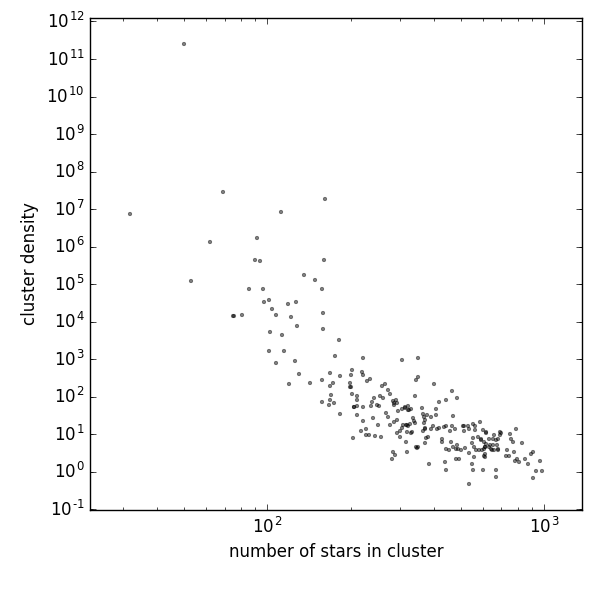
\includegraphics[width=2\figwidth]{./figs/clusters_0256.png}
\caption{The distribution of membership and density for the 256
  abundance-space clusters returned by the k-means algorithm at
  $K=256$.  The densest cluster---which is shown in
  \figurename~\ref{fig:M13}---is far more dense than the second
  densest.\label{fig:densities}}
\end{figure}
\begin{figure}[!p]
\insanefigure{cluster_0256_0253}
\caption{Same as \figurename~\ref{fig:all} except that the entire
  sample has been made gray and the members of the most dense
  $K=256$ abundance-space clusters have been rendered as unique, prominent triangles.
  This cluster, which was identified only in abundance space (six
  projections of which are the top six panels in this \figurename),
  turns out to be dominated by the halo globular cluster
  M13.\label{fig:M13}}
\end{figure}
\begin{figure}[!p]
\insanefigure{cluster_0256_0034}
\caption{Same as \figurename~\ref{fig:M13} but for another dense
  abundance-space cluster.
  This one turns out to be dominated by the disrupting globular
  cluster Palomar 5.\label{fig:Pal5}}
\end{figure}
\begin{figure}[!p]
\insanefigure{cluster_0256_0177}
\caption{Same as \figurename~\ref{fig:M13} but for another dense
  abundance-space cluster.
  This one turns out to be dominated by the Sagittarius star
  cloud.\label{fig:Sgr}}
\end{figure}
\begin{figure}[!p]
\insanefigure{cluster_0256_0010}
\caption{Same as \figurename~\ref{fig:M13} but for another dense
  abundance-space cluster.
  This one turns out to be dominated by a high-velocity-dispersion
  structure in the Galaxy halo.\label{fig:halo}}
\end{figure}
\begin{figure}[!p]
\insanefigure{cluster_0256_0141}
\caption{Same as \figurename~\ref{fig:M13} but for another dense
  abundance-space cluster.
  This one turns out to be dominated by a very thin young stellar
  structure in the Galaxy disk.\label{fig:disk}}
\end{figure}

\clearpage
\section{Discussion}

We have demonstrated for the first time that, in a large-scale
spectroscopic survey of stars, stars that appear similar in
chemical-abundance properties are often associated physically in
clusters or other structures.
The reverse is well established---that is, that stars that are
associated physically in clusters are similar in chemical-abundance
properties (with a recent model-free test by \citealt{bovy}).
MKN: WHAT ELSE TO CITE HERE?
However, it was not known whether abundance-space information would be
precise enough, or \emph{measurable} precisely enough to find this
structure in surveys dominated by a large mix of stars from different
origins and ages (and there was good reason to be pessimistic;
\citealt{ting}).
We have demonstrated with a straightforward (and in no way optimal)
clustering in chemical-abundance space that it is easy to find co-eval
stellar structures.

What made this possible is substantial improvements in precision
delivered by \thecannon.
We don't have an absolute measure of the precision of the measurements,
but from looking at open and globular clusters, it appears to be on the
order of or better than 0.04~dex for the median element in the list of 15.
These improvements are discussed in detail in the companion papers
\citep{casey16, ness16} about the abundance measurements.
We believe these improvements come from a combination of factors, not
limited to (a)~improvements in the determination of pseudo-continuum,
(b)~the use of more spectral range than just unblended element windows
\citep{aspcap}, and (c)~accurate spectral predictions
(\thecannon\ delivers accurate predictions because it is fit to
observed data).
Furthermore, because abundance space is high in dimensionality, even
small improvements in abundance measurement get taken to a significant
power when thinking about information gains.

ARC: Which known clusters were detected? Which comparably-sized clusters
	were not detected? Why not? (Why not M 15?)
	
ARC: How do the abundances that we find in these known clusters compare
	with the literature?

ARC: Expand on why these particular abundance projections, with
	comparisons to the literature.

ARC: We should note that the anti-correlations known to exist in GCs
	actually make this a *HARDER* task, since the abundances are
	somewhat arbitrarily structured (rather than normally concentrated)
	in a multi-dimensional space.

ARC: What can be said about the M 53 stars? Since we find GCs which are
	mostly spatially concentrated (e.g., very few sitting elsewhere),
	and then we find M53 "co-cluster" stars all over the halo, does this
	directly speak for evidence of accretion by proto-stellar clusters
	in the high-redshift analogues of the Milky Way?
	
ARC: In addition to the increased precision, it is very important to
	mention the fact that we report an "abundance" for *everything*.
	Gaps in abundance data from classical spectroscopy are rampant,
	and pose a serious problem even if you want to perform Real World(tm)
	tests of chemical tagging. \thecannon\ has solved this entire
	subset of astronomy.

There is no sense at all in which \figurename~\ref{fig:M13},
\ref{fig:Pal5}, \ref{fig:Sgr}, \ref{fig:halo}, and \ref{fig:disk} show
a representative or complete set of features found in abundance space.
These features were hand-chosen to be obviously interesting and
interpetable.
There are many other things to be found in this data set!

On the particulars of these features, a few comments:
DWH: Comments about Sag and M13: They appear in multiple clusters.
MKN: Comments about the young disk feature and what it probably is?

The \apogee\ project shows great promise for these studies, and with
the appearance of the companion papers, we will release the
chemical-abundance measurements we used here for further study.
The future is even brighter, however: \apogee\ is expanding to 19
elements, more stars, and all-sky angular coverage with \apogee2, and
\galah\ is nearly ready to release chemical abundances on a larger set
of 29 elements.
The \apogee\ elements employed in this project include alpha
(Mg, O, Si, Ca, Ti), light proton-capture (C, N, S), odd-Z (Na, Al, K)
and iron peak (Fe, Ni, V, Mn) elements.
\galah\ will deliver element abundances from all the major
nucleosynthetic processes, including light proton capture elements,
alpha, odd-Z, iron-peak, light and heavy slow neutron capture, and
rapid neutron capture.
Chemical tagging capabilities are expected to grow as the
\emph{product} of the measured nucleosynthetic pathways.

\acknowledgements
It is a pleasure to thank
  Jeremy Magland (\acronym{SCDA}), and
  Eddie Schlafly (\acronym{LBNL})
for valuable discussions.
This project was funded in part by
  the \acronym{NSF} (grants \acronym{IIS-1124794}, \acronym{AST-1517237}),
  \acronym{NASA} (grant \acronym{NNX12AI50G}),
  the Moore-Sloan Data Science Environment at \acronym{NYU}, and
  the European Research Council under the
  European Union's Seventh Framework Programme (FP~7)
  \acronym{ERC} Grant Agreement n.~\acronym{[320360, 321035]}).
This research made use of the \acronym{NASA} \project{Astrophysics Data System}.

This project made use of \sdssiii\ data.
Funding for \sdssiii\ has been provided by the Alfred P. Sloan
Foundation, the Participating Institutions, the National Science
Foundation, and the \acronym{U.S.} Department of Energy Office of Science. The
\sdssiii\ web site is http://www.sdss3.org/.

\sdssiii\ is managed by the Astrophysical Research Consortium for the
Participating Institutions of the \sdssiii\ Collaboration including the
University of Arizona, the Brazilian Participation Group, Brookhaven
National Laboratory, Carnegie Mellon University, University of
Florida, the French Participation Group, the German Participation
Group, Harvard University, the Instituto de Astrofisica de Canarias,
the Michigan State/Notre Dame/\acronym{JINA} Participation Group, Johns Hopkins
University, Lawrence Berkeley National Laboratory, Max Planck
Institute for Astrophysics, Max Planck Institute for Extraterrestrial
Physics, New Mexico State University, New York University, Ohio State
University, Pennsylvania State University, University of Portsmouth,
Princeton University, the Spanish Participation Group, University of
Tokyo, University of Utah, Vanderbilt University, University of
Virginia, University of Washington, and Yale University.

All of the code for the data manipulation, clustering, and
visualization is built on \project{numpy} \citep{numpy},
\project{scikit-learn} \citep{sklearn}, and \project{matplotlib}
\citep{matplotlib}.
All of the code written specifically for this project is available in
two open-source code repositories at
\url{https://github.com/andycasey/AnniesLasso} and
\url{https://github.com/davidwhogg/Platypus}.

\clearpage
\begin{thebibliography}{24}\raggedright
\bibitem[Alam \etal(2015)]{dr12}
Alam,~S., Albareti,~F.~D., Allende~Prieto,~C., \etal, 2015, \apjs, 219, 12
\bibitem[Bishop(2006)]{bishop}
Bishop,~C.~M., 2006, \textit{Pattern Recognition and Machine Learning}, Springer, New York
\bibitem[Blanco-Cuaresma \etal(2015)]{blancocuaresma}
Blanco-Cuaresma,~S., Soubiran,~C., Heiter,~U., \etal, 2015, \aap, 577, A47
\bibitem[Bovy(2015)]{bovy}
Bovy,~J., 2015, arXiv:1510.06745
\bibitem[Casey \etal(2016)]{casey16}
Casey,~A.~R., Hogg,~D.~W., Ness,~M., Rix,~H.-W., 2016, in preparation
\bibitem[De~Silva \etal(2015)]{galah}
De~Silva,~G.~M., Freeman,~K.~C., Bland-Hawthorn,~J., \etal, 2015, \mnras, 449, 2604
\bibitem[Font \etal(2006)]{font}
Font,~A.~S., Johnston,~K.~V., Bullock,~J.~S., Robertson,~B.~E., 2006, \apj, 638, 585 
\bibitem[Freeman \& Bland-Hawthorn(2002)]{freeman}
Freeman,~K., Bland-Hawthorn,~J., 2002, \araa, 40, 487
\bibitem[Garc{\'{\i}}a~P{\'e}rez \etal(2015)]{aspcap}
Garc{\'{\i}}a~P{\'e}rez,~A.~E., Allende~Prieto,~C., Holtzman,~J.~A., \etal, 2015, arXiv:1510.07635
\bibitem[Gilmore et al.(2012)]{gaiaeso} Gilmore, G., Randich, 
S., Asplund, M., et al.\ 2012, The Messenger, 147, 25 
\bibitem[Hunter(2007)]{matplotlib}
Hunter,~J.~D., 2007, Computing in Science \& Engineering, 9, 90
\bibitem[Jofr{\'e} \etal(2015)]{jofre} Jofr{\'e}, P., 
M{\"a}dler, T., Gilmore, G., et al.\ 2015, \mnras, 453, 1428 
\bibitem[Majewski \etal(2015)]{apogee}
Majewski,~S.~R., Schiavon,~R.~P., Frinchaboy,~P.~M., \etal, 2015, arXiv:1509.05420
\bibitem[Martell(2015)]{martell}
Martell,~S.~L., 2015, arXiv:1507.00079
\bibitem[Melendez \etal(2014)]{melendez}
Mel{\'e}ndez,~J., Ram{\'{\i}}rez,~I., Karakas,~A.~I., \etal, 2014, \apj, 791, 14
\bibitem[Mitschang \etal(2014)]{mitschang}
Mitschang,~A.~W., De~Silva,~G., Zucker,~D.~B., \etal, 2014, \mnras, 438, 2753
\bibitem[Ness \etal(2015)]{thecannon}
Ness,~M., Hogg,~D.~W., Rix,~H.-W., Ho,~A.~Y.~Q., Zasowski,~G., 2015, \apj, 808, 16
\bibitem[Ness \etal(2016a)]{ages}
Ness,~M., Hogg,~D.~W., Rix,~H.-W., \etal, 2016a, \apj, in press (arXiv:1511.08204)
\bibitem[Ness \etal(2016b)]{ness16}
Ness,~M., Hogg,~D.~W., Casey,~A.~R., Rix,~H.-W., 2016b, in preparation
\bibitem[Pedregosa \etal(2011)]{sklearn}
Pedregosa,~F., Varoquaux,~G., Gramfort,~A., \etal, 2011, Journal of Machine Learning Research, 12, 2825
\bibitem[Quillen \etal(2015)]{quillen}
Quillen,~A.~C., Anguiano,~B., De~Silva,~G., \etal, 2015, \mnras, 450, 2354
\bibitem[Ro{\v s}kar \etal(2008)]{roskar}
Ro{\v s}kar,~R., Debattista,~V.~P., Quinn,~T.~R., Stinson,~G.~S., Wadsley,~J., 2008, \apjl, 684, L79
\bibitem[Ting \etal(2016)]{ting}
Ting,~Y.-S., Conroy,~C., Rix,~H.-W., 2016, \apj, in press (arXiv:1507.07563)
\bibitem[van~der~Walt \etal(2011)]{numpy}
van~der~Walt,~S., Colbert,~S.~C., Varoquaux,~G., 2011, Computing in Science \& Engineering, 13, 22
\end{thebibliography}
\end{document}
